%%%%%%%%%%%%%%%%%%%%%%%%%%%%%%%%%%%%%%%%%%%%%%%%%%%%%
% SPARSE SYNTHETIC CONTROL
%%%%%%%%%%%%%%%%%%%%%%%%%%%%%%%%%%%%%%%%%%%%%%%%%%%%%
\subsection{Sparse Synthetic Control}

The core component of our pairs trading strategy involves constructing a synthetic asset that replicates the log-price behavior of a target security using a sparse linear combination of assets from a donor pool. 
%
Let $\mathcal T$ denote the collection of timestamps of a sample, with $T:=\card{\mathcal T}$. This sample is divided into training and test samples: $\mathcal T=\mathcal T_{tr} \cup \mathcal T_{test}$.
%\footnote{Throughout the text, we will indisctinctively refer to the training sample as \qquote{estimation sample} or as \qquote{in-sample}. Analogously, we will refer to the test sample as the \qquote{evaluation sample} or more succintly, \qquote{out-of-sample}}
%
Let $\mbf y = [y_{t}]_{t=1}^T\in \R^{T}$ denote the log-price time series of a target asset and $\mbf X = [x_{1t}, ..., x_{Nt}]_{t=1}^T\in\R^{T\times N}$ denote the log-price time series of a donor pool of $N$ assets. Then, we can build a synthetic log-price time series ${\mbf y}^*\in \mathbb{R}^T$ as:
\begin{equation*}
%{y}_{t}^* = \sum_{i=1}^N w_i^* x_{it}
%\quad \text{for~} t=1,...,T
%,
\mbf y^* = \mbf X \mbf w^*
\end{equation*}

where the weights $\mbf w^*=[w_1^*, ..., w_N^*]\'\in \R^N$ are determined in-sample via an $\ell_1$-regularized least squares optimization problem
%----------------------------------------------------
\begin{equation*}
\mathbf{w}^* 
= \argmin_{\mathbf{w} \in \R^{N}} \left\{\sum_{t\in\mathcal T_{tr}} \left(y_{t} - \sum_{i=1}^N w_i x_{it}\right)^2 + \lambda\|\mathbf{w}\|_1\right\}
\quad \text{s.t.} \quad \mathbf{1}^\top \mathbf{w} = 1
\end{equation*}
%----------------------------------------------------
%\begin{equation*}
%\mathbf{w}^* 
%= 
%\2{
%\begin{array}{cl}
%\underset{\mathbf{w} \in \R^{N}}{\arg\min} &
%\sum_{t=1}^T \left(y_{t} - \sum_{i=1}^N w_i x_{it}\right)^2 
%%\norm{\mbf y - \mbf {Xw}}_2^2
%+ \lambda\|\mathbf{w}\|_1
%\\
%\text{s.t.} & \mathbf{1}^\top \mathbf{w} = 1
%\end{array}
%}
%\end{equation*}
%----------------------------------------------------

where $\|\mathbf{w}\|_1 = \sum_{i=1}^N |w_i|$ denotes the $\ell_1$-norm of the weight vector, $\lambda > 0$ is a regularization parameter that controls the level of sparsity.
%This formulation promotes sparse solutions through the $\ell_1$ penalty term while maintaining the constraint that the weights sum to unity. 
The $\ell_1$ regularization, also known as the lasso penalty, induces sparsity by shrinking some weights exactly to zero, effectively performing feature selection among the donor assets. This sparsity-inducing property stems from the non-differentiability of the penalty term at the origin. %\cite{tibshirani1996regression}.
The practical implementation of this procedure is given in \cref{alg:synthetic_control}

The optimization problem possesses several key theoretical and practical features that make it particularly suitable for our application. First, the combination of a quadratic loss function with the convex $\ell_1$-penalty and affine constraint guarantees a unique solution under mild regularity conditions. % \cite{boyd2004convex}.
Second, the regularization parameter $\lambda$ (optimally selected through cross-validation) provides direct control over the sparsity level, with larger values yielding solutions with fewer non-zero weights. Third, the simplex constraint $\mbf 1^\top \mbf w = 1$ ensures interpretability of the synthetic control as a weighted portfolio of donor assets. We don't impose a convex hull restriction, which effectively means that we allow for negative ways in the synthetic asset.

The resulting weight vector $\mathbf{w}^*$ will typically have many components equal or very close to zero, with the number of non-zero weights decreasing as $\lambda$ increases. In practice, we identify the support of non-zero weights through thresholding:
\begin{equation*}
\mathcal{I} = \{i \in \{1,...,N\} : |w^*_i| > \epsilon\}
\end{equation*}
where $\epsilon > 0$ is a small tolerance threshold (in our application, $\epsilon \approx 10^{-5}$). The final synthetic asset is then constructed using only assets in $\mathcal{I}$. We chose to sparsify the synthetic control using lasso instead of solving a cardinality-constrained program as the former is able to maintain sparse exposures while enjoying vast computational advantages. Moreover, the convex nature of the problem permits efficient solution via proximal algorithms or quadratic programming techniques, making it suitable for high-dimensional donor pools. For a detailed discussion, see \cref{sec:discussion_card_constr}.


The reader may draw similarities of this process with the Engle-Granger procedure for estimating the cointegration vector associated to the target asset and the donor pool. If we don't impose the $\ell_1$-penalty, it can be shown that, under some conditions, the procedure of finding the weights of the synthetic control is equivalent to finding the cointegration vector. For a formal discussion see \cref{sec:cointegration_meets_synthetic_controls}.


%==============[	  Empirical Application  ]==============
%For the empirical application, we will use daily adjusted-close stock price data from the S\&P500. For illustration, we will set NVIDIA as our target stock and leave all the rest stocks in the donor pool. We have data from January 2010 to January 2025. We divide it into training ($70\%$) and test set ($30\%$) and obtain the synthetic control weights from the training sample. This delivers the weights shown in \cref{tab:scm_weights}. As we can see, our synthetic control is composed of 27 stocks with weights that sum to 1. Some weights are positive, indicating a long position, and others are negative, indicating a short position. 
%This sparse portfolio structure effectively defines a tradeable basket that can be executed simultaneously through standard ETF-like basket trading mechanisms.
%This synthetic control defines a \qquote{basket} that is to be traded at unison in an ETF-like style.

To evaluate our methodology empirically, we implement the synthetic control approach using daily adjusted-close price data from S\&P500 constituents. We select NVIDIA (NVDA) as our target asset and construct the donor pool from the remaining index components. The full sample runs from January 2010 to January 2025 and is partitioned chronologically, with 70\% allocated to the training period for model estimation and the remaining 30\% reserved for out-of-sample testing. The optimization procedure detailed in the previous section yields the optimal weights presented in \cref{tab:scm_weights}. The resulting synthetic control comprises 27 stocks with non-zero weights that sum to unity, distributed between long positions (positive weights) and short positions (negative weights). This sparse portfolio structure effectively defines a tradeable basket that can be executed simultaneously through standard ETF-like basket trading mechanisms.

%==============[	  Table 1 ]==============
\begin{table}[H] 
\centering
\caption{Synthetic Control Model Weights}
\label{tab:scm_weights}
\begin{tabular}{llc}
\toprule
 Tickers & Company Name & Weights (\%) \\
\midrule
\textbf{AME} & Ametek & 41.08 \\
\textbf{LUV} & Southwest Airlines & 33.31 \\
\textbf{TFC} & Truist Financial & 25.60 \\
\textbf{AEP} & American Electric Power & 21.69 \\
\textbf{ADM} & Archer Daniels Midland & 20.56 \\
\textbf{RSG} & Republic Services & 18.42 \\
\textbf{AXP} & American Express & 18.10 \\
\textbf{LLY} & Lilly (Eli) & 14.74 \\
\textbf{C} & Citigroup & 9.67 \\
\textbf{VRSN} & Verisign & 7.77 \\
\textbf{MTB} & M\&T Bank & 7.38 \\
\textbf{FE} & FirstEnergy & 7.16 \\
\textbf{FIS} & Fidelity National Information Services & 5.21 \\
\textbf{PARA} & Paramount Global & 4.48 \\
\textbf{TXT} & Textron & 2.21 \\
\textbf{STX} & Seagate Technology & 0.26 \\
\textbf{BIIB} & Biogen & 0.16 \\
\textbf{NFLX} & Netflix & -1.04 \\
\textbf{FDX} & FedEx & -2.39 \\
\textbf{UDR} & UDR, Inc. & -3.95 \\
\textbf{V} & Visa Inc. & -5.43 \\
\textbf{CNP} & CenterPoint Energy & -7.75 \\
\textbf{MS} & Morgan Stanley & -16.21 \\
\textbf{NI} & NiSource & -16.35 \\
\textbf{WMT} & Walmart & -16.65 \\
\textbf{UNP} & Union Pacific Corporation & -25.77 \\
\textbf{ADSK} & Autodesk & -42.25 \\
\bottomrule
 & Total& 100.00 \\
\bottomrule
\end{tabular}

%----------------------------------------------------
\vspace{0.5cm}
\begin{minipage}{\textwidth}
\setlength{\parindent}{0pt}
\small\textit{Note: 
% Optimal weights of the sparse synthetic control portfolio for replicating the target asset's price dynamics. The table displays the percentage contribution of each donor asset from the S\&P 500 constituents, with positive weights indicating long positions and negative weights indicating short positions. The weights are derived using an $\ell_1$-regularized least squares optimization, which enforces sparsity by shrinking some weights to zero, effectively selecting the most influential assets. The weights sum to 100\% as enforced by the simplex constraint in the optimization problem.
This table presents the optimal weights obtained from the sparse synthetic control methodology for replicating the target asset's price dynamics. The weights are expressed as percentages and represent each donor asset's contribution to the synthetic portfolio. Positive weights indicate long positions while negative weights represent short positions. The donor pool consists of S\&P 500 constituents, and the methodology yields a sparse solution where many potential donor assets receive zero weights. The sparsity is achieved through $\ell_1$-regularization, which automatically selects the most influential assets for constructing the synthetic control. The weights sum to 100\% as enforced by the simplex constraint in the optimization problem.
}
\end{minipage}
%----------------------------------------------------
\end{table}


%%%%%%%%%%%%%%%%%%%%%%%%%%%%%%%%%%%%%%%%%%%%%%%%%%%%%
%%%%%%%%%%%%%%%%%%%%%%%%%%%%%%%%%%%%%%%%%%%%%%%%%%%%%
%\inserthere{tab:scm_weights}
%\begin{table}[H] 
%\centering
%\caption{Synthetic Control Model Weights}
%\label{tab:scm_weights}
%\begin{tabular}{cc}
%\toprule
% Tickers & Weights (\%) \\
%\midrule
%\textbf{AME} & 41.08 \\
%\textbf{LUV} & 33.31 \\
%\textbf{TFC} & 25.60 \\
%\textbf{AEP} & 21.69 \\
%\textbf{ADM} & 20.56 \\
%\textbf{RSG} & 18.42 \\
%\textbf{AXP} & 18.10 \\
%\textbf{LLY} & 14.74 \\
%\textbf{C} & 9.67 \\
%\textbf{VRSN} & 7.77 \\
%\textbf{MTB} & 7.38 \\
%\textbf{FE} & 7.16 \\
%\textbf{FIS} & 5.21 \\
%\textbf{PARA} & 4.48 \\
%\textbf{TXT} & 2.21 \\
%\textbf{STX} & 0.26 \\
%\textbf{BIIB} & 0.16 \\
%\textbf{NFLX} & -1.04 \\
%\textbf{FDX} & -2.39 \\
%\textbf{UDR} & -3.95 \\
%\textbf{V} & -5.43 \\
%\textbf{CNP} & -7.75 \\
%\textbf{MS} & -16.21 \\
%\textbf{NI} & -16.35 \\
%\textbf{WMT} & -16.65 \\
%\textbf{UNP} & -25.77 \\
%\textbf{ADSK} & -42.25 \\
%\bottomrule
%\textbf{Total} & 100.00 \\
%\bottomrule
%\end{tabular}
%
%%----------------------------------------------------
%\vspace{0.5cm}
%\begin{minipage}{\textwidth}
%\setlength{\parindent}{0pt}
%\small\textit{Note: 
%% Optimal weights of the sparse synthetic control portfolio for replicating the target asset's price dynamics. The table displays the percentage contribution of each donor asset from the S\&P 500 constituents, with positive weights indicating long positions and negative weights indicating short positions. The weights are derived using an $\ell_1$-regularized least squares optimization, which enforces sparsity by shrinking some weights to zero, effectively selecting the most influential assets. The weights sum to 100\% as enforced by the simplex constraint in the optimization problem.
%This table presents the optimal weights obtained from the sparse synthetic control methodology for replicating the target asset's price dynamics. The weights are expressed as percentages and represent each donor asset's contribution to the synthetic portfolio. Positive weights indicate long positions while negative weights represent short positions. The donor pool consists of S\&P 500 constituents, and the methodology yields a sparse solution where many potential donor assets receive zero weights. The sparsity is achieved through $\ell_1$-regularization, which automatically selects the most influential assets for constructing the synthetic control. The weights sum to 100\% as enforced by the simplex constraint in the optimization problem.
%}
%\end{minipage}
%%----------------------------------------------------
%\end{table}



The time series evolution of the target and synthetic log-prices is shown in \cref{fig:target_synthetic_prices_NVDA}. As we can see, the fit is really good in the training sample, but as we move out of sample, the spread between the two series becomes more volatile and the two series seem to diverge in recent years. As we will see later, we should not worry too much about the log-price fit, as the trading strategy capitalizes on the mean-reversion of returns (rather than log-prices).

%==============[	  Figure 1  ]==============
\inserthere{fig:target_synthetic_prices_NVDA}
\begin{figure}[H]
  \caption{Target vs Synthetic Log-Prices for NVDA}
  \centering
  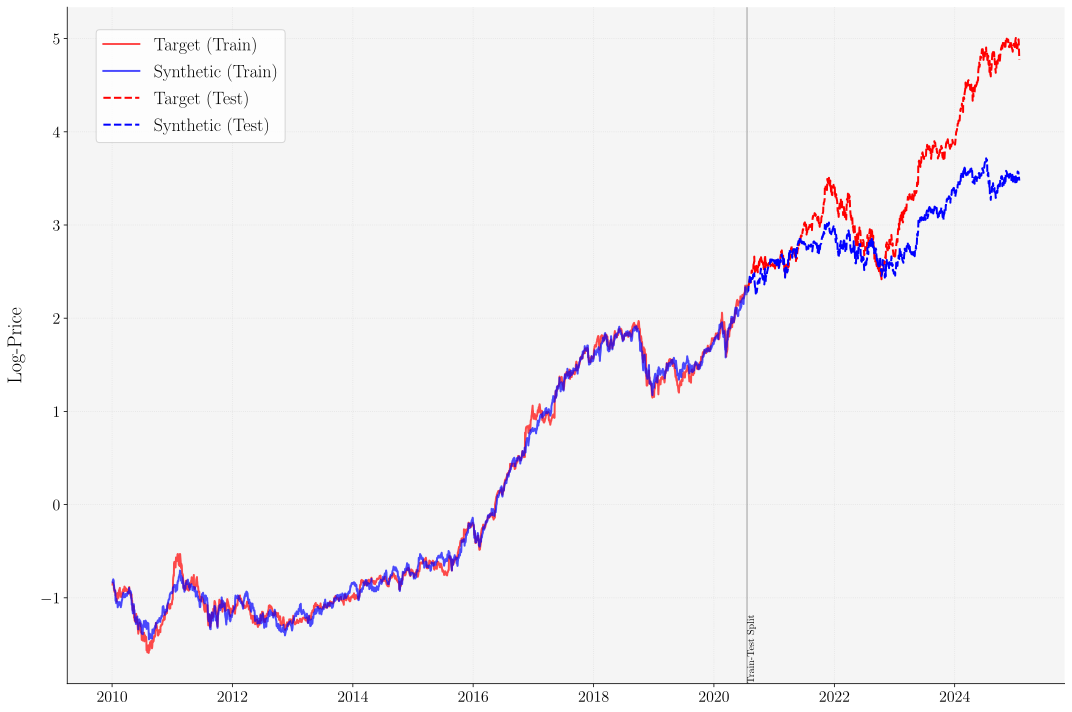
\includegraphics[scale=0.47]{/Users/jesusvillotamiranda/Library/CloudStorage/OneDrive-UniversidaddeLaRioja/GitHub/Repository/arbitragelab-master/__OUTPUT_TeX__/figures/target_synthetic_prices_NVDA.pdf}
\label{fig:target_synthetic_prices_NVDA}
%.............
\vspace{0.5cm}
\begin{minipage}{\textwidth}
\setlength{\parindent}{0pt}
\small\textit{Note: 
This figure illustrates the log-price trajectories of the target asset (NVDA) and its synthetic counterpart over the training and testing periods. The solid blue line represents the synthetic log-prices derived from the sparse synthetic control methodology, while the solid red line indicates the actual log-prices of the target asset during the training phase. The dashed lines depict the log-prices for both the target and synthetic assets during the testing phase. The vertical line marks the transition point between the training and testing datasets
}
\end{minipage}
%.............
\end{figure}

